% Lecture Template for ENGR 1120 030 031 E01- Tristan Hill - Spring 2017m - Fall 2017
% 
% Introduction to MATLAB 
%
% Intro to Looping and Repetition

% Document settings
\documentclass[11pt]{article}
\usepackage[margin=1in]{geometry}
\usepackage[pdftex]{graphicx}
\usepackage{multirow}
\usepackage{setspace}
\usepackage{hyperref}
\usepackage{color,soul}
\usepackage{fancyvrb}
\usepackage{framed}
\usepackage{wasysym}
\usepackage{multicol}

\pagestyle{plain}
\setlength\parindent{0pt}
\hypersetup{
    bookmarks=true,         % show bookmarks bar?
    unicode=false,          % non-Latin characters in Acrobat’s bookmarks
    pdftoolbar=true,        % show Acrobat’s toolbar?
    pdfmenubar=true,        % show Acrobat’s menu?
    pdffitwindow=false,     % window fit to page when opened
    pdfstartview={FitH},    % fits the width of the page to the window
    pdftitle={My title},    % title
    pdfauthor={Author},     % author
    pdfsubject={Subject},   % subject of the document
    pdfcreator={Creator},   % creator of the document
    pdfproducer={Producer}, % producer of the document
    pdfkeywords={keyword1} {key2} {key3}, % list of keywords
    pdfnewwindow=true,      % links in new window
    colorlinks=true,       % false: boxed links; true: colored links
    linkcolor=red,          % color of internal links (change box color with linkbordercolor)
    citecolor=green,        % color of links to bibliography
    filecolor=magenta,      % color of file links
    urlcolor=blue           % color of external links
}

% assignment number 
\newcommand{\NUM}{5 } 
\newcommand{\VSpaceSize}{2mm} 
\newcommand{\HSpaceSize}{2mm} 

\definecolor{mygray}{rgb}{.6, .6, .6}

% [153,50,204] - dark orchid
\definecolor{mypurple}{rgb}{0.6,0.1961,0.8}
%[139,69,19] - saddle brown
\definecolor{mybrown}{rgb}{0.5451,0.2706,0.0745}
\definecolor{mygreen}{rgb}{0,.4,0}


\setulcolor{red} 
\setstcolor{green} 
\sethlcolor{mygray} 

\newcommand{\R}{\color{red}}
\newcommand{\B}{\color{blue}}
\newcommand{\K}{\color{black}}
\newcommand{\GR}{\color{mygreen}}
\newcommand{\PR}{\color{mypurple}}
\newcommand{\BR}{\color{mybrown}}


\begin{document}

\textbf{ \LARGE ENGR 1120 Lecture Chapter \NUM - Looping Statements } \\
	
%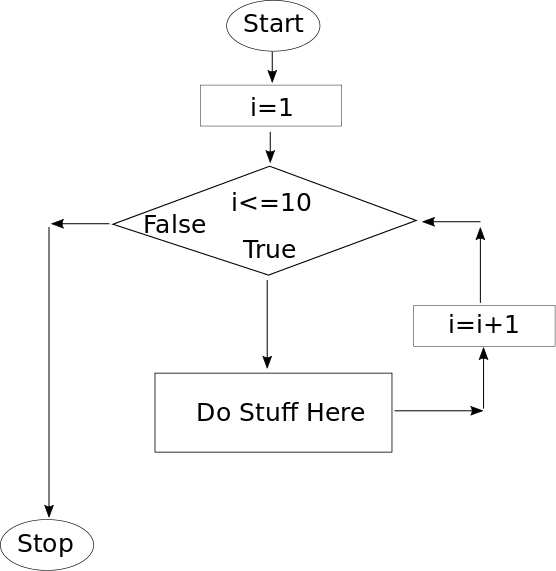
\includegraphics[scale=0.3]{lecture1_fig1.png}\\\\

\Large
\begin{itemize}


	
	\item \textbf{ \LARGE What is \color{mypurple}Looping \color{black}? Why \color{mypurple}Loop\color{black} ?}\\
	
	\begin{itemize}
	\item \textbf{ \LARGE Have you noticed that in your previous programs\\\\ that there was alot of  \color{mypurple}Repeated Code \color{black}? }\\\\\\
	
	\item \textbf{ \LARGE Why is alot of \color{mypurple}Repeated Code \color{black} bad? }\\
	\begin{itemize}
	\item \vspace{10mm}
	\item \vspace{10mm}
	\item \vspace{10mm}
	\end{itemize}
	
	\vspace{10mm}
			\item \textbf{ \LARGE What can we do about it?  }\vspace{30mm}\\
            			
            		\item \textbf{ \LARGE Introduce a new \color{blue}Control Structure \color{black} ... }\vspace{30mm}\\
		\end{itemize}
\newpage

	\item \textbf{ \LARGE the \color{mypurple}While Loop \color{black}is a \color{blue}Control Structure \color{black} used for\\ repeating code}\\
\begin{itemize}
	\item \textbf{ \Large in MATLAB this requires the \color{mypurple} reserved keywords \color{black} \color{blue}while  \color{black} and \color{blue}end \color{black}}\vspace{5mm} \\
	
	\item \textbf{ \Large everything between  \color{black} \color{blue}while  \color{black} and \color{blue}end \color{black} is {\BR repeated} as long as the \color{mybrown} condition \color{black} is true }\vspace{5mm} \\


\item \textbf{ \Large the \color{mybrown} condition \color{black} that controls the loop is a \color{mypurple}Logical Statment} \color{black} \vspace{10mm} \\

\item \textbf{ \Large looping structures can be \color{mypurple} nested \color{black} as well}\vspace{10mm} \\

\end{itemize}
	\item \textbf{\LARGE  Now we can  \color{mypurple}Design \color{black} more complex \color{blue}Program Flow \color{black}}\\

				\newpage
				\item \textbf{\LARGE Flowchart Representation}\\\\
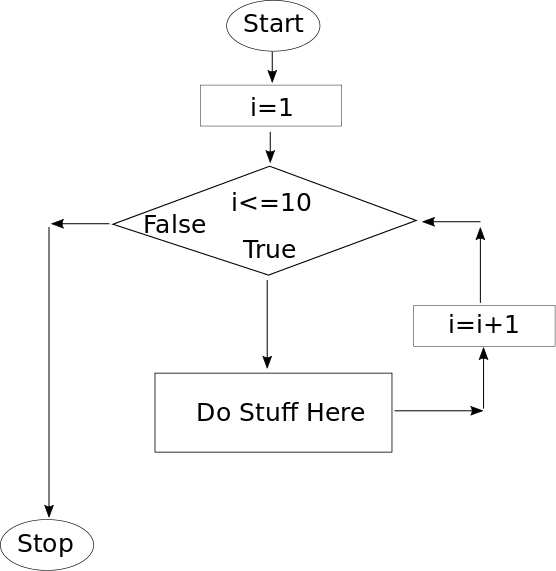
\includegraphics[scale=0.6]{lecture1_fig1.png}\\	

				\item \textbf{\LARGE MATLAB \color{mypurple} syntax \color{black}}\\
\begin{framed}				
						 \scalebox{1.1}{{\fontfamily{qcr}\selectfont \color{black}i=1; \color{mygreen}\%Initialize the loop counter\color{black}}} \\\\
						 \scalebox{1.1}{{\fontfamily{qcr}\selectfont \color{blue}while \color{black} (i<=10) }} \\\\
						 \hspace*{10mm}\scalebox{1.1}{{\fontfamily{qcr}\selectfont \color{mygreen}\%Do Stuff Here\color{black} }} \\\\
						 \hspace*{10mm}\scalebox{1.1}{{\fontfamily{qcr}\selectfont \color{black}i=i+1; \color{mygreen}\%Increment the loop counter\color{black} }} \\\\
						 \scalebox{1.1}{{\fontfamily{qcr}\selectfont \color{blue}end\color{black} }} \\		
\end{framed}
			
				\newpage
				
\item \textbf{ \LARGE Introduction to \color{mypurple} Algorithms \color{black}}\\
{\LARGE
\begin{itemize}
	\item ``In mathematics and computer science, an algorithm is a self-contained sequence of actions to be performed. Algorithms perform calculation, data processing, and/or automated reasoning tasks.'' - Wikipedia\vspace{10mm}
	\item ``A step by step description of a process'' - me\vspace{10mm}
	\item ``A solution technique for a {\it general problem}'' - me\vspace{10mm}
	\end{itemize}
	}
	\item \textbf{ \LARGE Basic \color{mypurple} Algorithms \color{black} every programmer needs}\\
	{\LARGE
	\begin{itemize}
	\item count \vspace{10mm}
	\item sum  \vspace{10mm}
	\item average  \vspace{10mm}
	\item maximum  \vspace{10mm}
	\item minimum  \vspace{10mm}
	\end{itemize}
	}
				\newpage
				\item \textbf{ \LARGE \color{mypurple} Counting \color{black}}\\
	
				\newpage
				\item \textbf{ \LARGE \color{mypurple} Summation \color{black} and \color{mypurple} Average \color{black}}\\
				\newpage
				\item \textbf{ \LARGE \color{mypurple} Maximum \color{black} and \color{mypurple} Minimum \color{black}}\\
\end{itemize}


	

\end{document}



